\uuid{VHrA}
\exo7id{7155}
\titre{exo7 7155}
\auteur{megy}
\organisation{exo7}
\datecreate{2017-05-13}
\isIndication{true}
\isCorrection{true}
\chapitre{Géométrie affine euclidienne}
\sousChapitre{Géométrie affine euclidienne du plan}

\contenu{
\texte{
% composition de similitudes
% hauteurs, orthocentre
Soit $ABC$ un triangle direct non rectangle isocèle, et soit $P$ (resp. $Q$, $R$) tel que $BCP$ (resp. $CAQ$, $ABR$) soit direct isocèle rectangle en $P$ (resp. $Q$ et $R$). 

\begin{center}
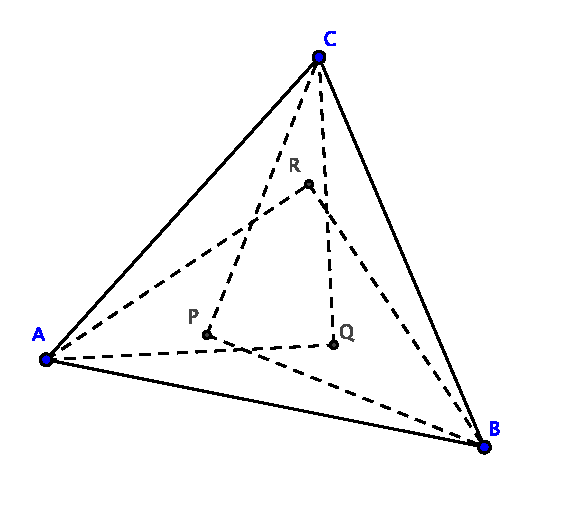
\includegraphics{../images/img007155-1}
\end{center}
}
\begin{enumerate}
    \item \question{Montrer que $\overrightarrow{AP}$ et $\overrightarrow{QR}$ sont orthogonaux et de même norme.}
\reponse{Suivons l'indication. Soit $s = s_2\circ s_1$. C'est une similitude directe de rapport $1$ et d'angle $\pi/2$. On vérifie également que $s(C')=C'$, donc c'est la rotation de centre $C'$ et d'angle $\pi/2$. 

Or, d'une part on a  $s(R)=A$, et d'autre part $s_1(Q) = C$ et $s_2(C) = P$, donc $s(Q) = P$. On en déduit que $\overrightarrow{AP}$ est l'image de $\overrightarrow{RQ}$ par une rotation de $\pi/2$. Les vecteurs ont donc même norme et sont orthogonaux.}
    \item \question{Montrer que les droites $(AP)$, $(BQ)$ et $(CE)$ sont concourantes.}
\reponse{Les droites $(AP)$, $(BQ)$ et $(CE)$ sont les hauteurs de $PQR$ donc sont concourantes en l'orthocentre de $PQR$. Ce point est le \emph{point intérieur de Vecten} de $ABC$.}
\indication{Si on n'utilise pas les nombres complexes, on pourra considérer $C'$ le milieu de $[AB]$, $s_1$ la similitude directe de centre $A$, de rapport $\sqrt 2$ et d'angle $\pi/4$ et $s_2$ la similitude de centre $B$, de rapport $1/\sqrt 2$ et d'angle $\pi/4$.

Dans le contexte de cet exercice, les similitudes directes seront utilisées comme dans l'exemple suivant : comme AQC est rectangle isocèle en $Q$, la similitude directe de centre $A$, d'angle $\pi/4$ et de rapport $\sqrt 2$ envoie $Q$ sur $C$.}
\end{enumerate}
}
